\chapter{Design-Dokument}
\section{Einleitung}
Dieses Dokument dient der Darstellung der Gesamt-Architektur des Software-Projekts "Freya-MPD-Client"
Zunächst werden einige UML-Diagramme zur Übersicht gezeigt und anschließend einzelne Funktionen der
Software genauer unter die Lupe genommen.\ \\
Im Anschluss daran wird die Benutzeroberfläche präsentiert und in Bereiche aufgeteilt genauer dargestellt.
Dabei werden alle Schaltflächen und Info-Panel genau erläutert.
Anschließend folgt eine Übersicht zu allen Short-Cuts die genutzt werden können.
Danach werden einige Use-Case-Fälle angeschaut, um genau zu verstehen, wie die Software mit dem Nutzer
interagiert und auf Befehle reagiert.
\newpage
\section{Softwarearchitektur}
\subsection{Architekutrübersicht}
\subsubsection{Namespace-Übersicht}
\begin{figure}[h]
\centering
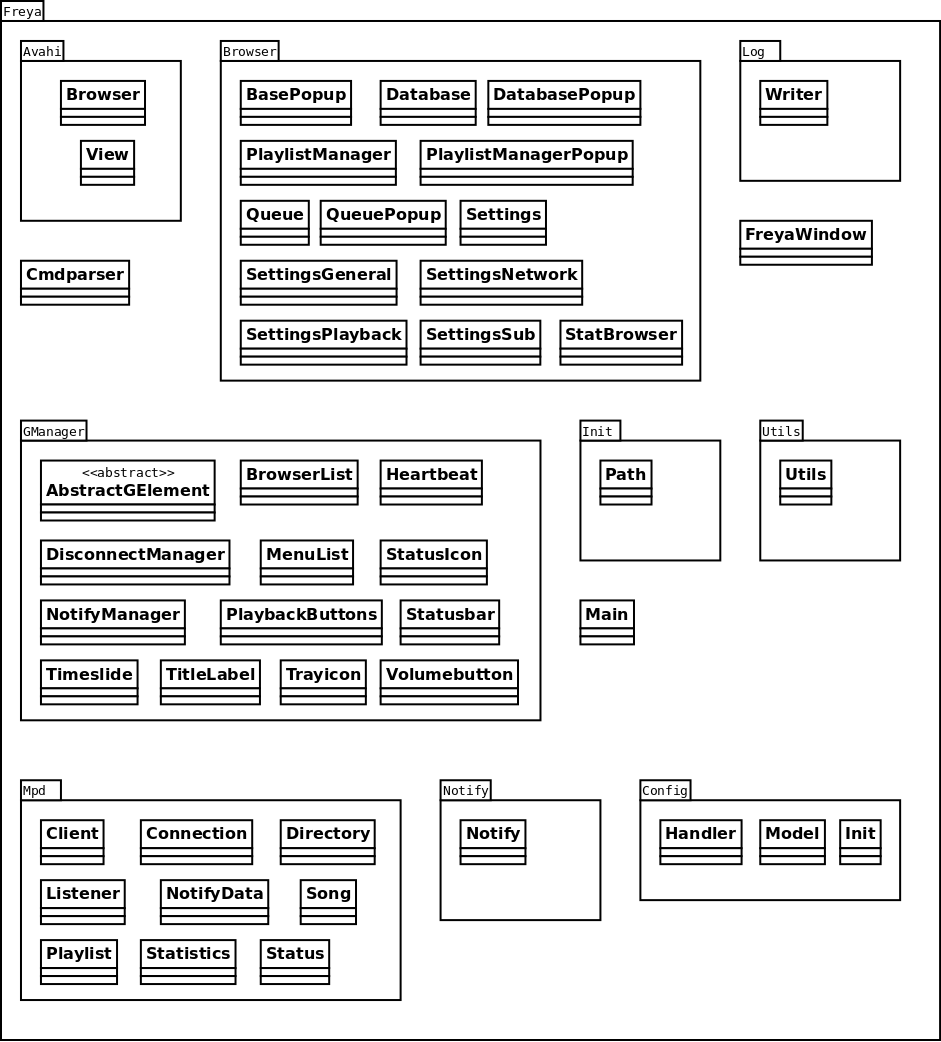
\includegraphics[scale=0.3]{Namespace_Uebersicht.png}
\end{figure}
\newpage
\subsubsection{Beschreibung}
\subsection{Funktionen}
\subsubsection{Beispiel-Abspielfunktionen}
\subsubsection{Beispiel-Playlist erstellen}
\subsubsection{Beispiel-Dateibrowser}
\subsection{Oberfläche}
\subsubsection{Titelleiste}
\subsubsection{Seitenmenü}
\subsubsection{Fußleiste}
\subsubsection{Anzeige}
\subsection{Short-Cuts}
\section{Use-Case-Fälle}
\subsection{Musik abspielen}
\subsection{Musik zufällig abspielen}
\subsection{Musik im Consume Mode abspielen}
\subsection{Playlist erstellen}

